\section{System and Security Model}
As shown in Fig. \ref{fig:model}, the proposed scheme works in a communication system with the following 4 kinds of entities: several Identity Providers (IdP) and Relying parties (RP), multiple users with their personal mobile equipments (UE), and a communication core network with specialized network elements (Fig. \ref{fig:model} uses the 5G system as an instance). The follows describe each of the entities. 

%The privacy-preserving multi-factor authentication protocol based on anonymous credential relies on two parties: an credential issuer and a Relying Party (RP). The issuer provides an anonymous credential to each user. A user registers for an SMS-relay service at the 5G system network. The credential is used by a registered user in authentication with third party applications, in other words Relying Parties (RP), that support our protocol. The services of the application will be accessible to the user after successful authentication with the RP. 

%The overall workflow of the authentication protocol is demonstrated in Fig[]. The protocol consists of three phases, namely Initialization, Registration, and Authentication. The credential for each user is issued in the Initiaization phase. The SMS-relay service of a user is registered in the second phase. And the multi-factor authentication is done in the third phase.

\begin{figure}[t]
	\centering
	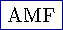
\includegraphics[width=6cm]{architecture}
	\caption{Architecture of the 2-Factor Authentication System}\label{fig:model}
\end{figure}

\subsection{Architectures}
\subsubsection{IdP (Identity providers)}
They are responsible for issuing credentials for other entities, like UE. In this paper, each credential claims a set of attributes, with the signature of the issuing IdPs. 

For different deployment models, a credential can be signed by a single, or multiple IdPs. The latter is more convenient from the perspective of both privacy and reliability. In later content, the construction is described as the one-IdP model, whereas, the extension to the multiple-IdP is straightforward.

\subsubsection{RP (Relying parties)}
They publish diverse services in the network platform. Each service can be accessed according to the RP's designated access policy $\mathcal{P}$. A policy is a predicate, containing a set of attribute values (or value ranges).

In a multi-IdP system, RP only accepts the UE, whose credential satisfies its policy, and signed by its trusted IdPs. Thus, RP will initialize trust relationship between IdPs.

\subsubsection{UE (User equipment)}
It is a concept in 3GPP system, which is an entity with mobile equipment (ME, generally the smart phones) and the USIM card. It can access two network: one the one hand, it can access data network (DN) via 5G data plain (as shown in Fig. \ref{fig:model}) or via other communication technology (e.g., WiFi); on the other hand, it accesses the network services directly provided by the 5G core systems, such as short message services (SMS), voice calls.

As each UE is owned by a user, it will register and request credential from some IdPs, with which, it can proves its privilege to the RPs to enjoy the services in the network. 

\subsubsection{5G Core}
It is a set of network elements provided by a network service provider (NSP). Readers who are interested in it can refer to 3GPP TS23.501 \cite{3gpp23501} to see the entire architecture, and Fig. \ref{fig:model} shows some of them, which relate to our construction. Especially, the UDM is in the domain of home agent, maintaining UE's subscription and context data; AMF is a core element for controlling plane; SMSF and SMS-GMSC are elements specific for short message services. Table \ref{tab:5G} depicts a more detailed introduction.

Return to the system model, the 5G core system is responsible for short message delivery for UE, to assist the multi-factor authentication between diverse RPs. It also has ability to undertake package relay for UE's Internet tasks.%, whereas, it is optional.

\begin{table}[t]
	\caption{Necessary Description for 5G Core}\label{tab:5G}
	\centering
	\begin{tabular}{c|p{6cm}}
		\hline
		\textbf{Notations} & \textbf{Description} \\
		\hline
		AMF & Access and Mobility Management Function, it supports necessary controlling plane signals, e.g., device authentication, paging, and SMS over NAS.\\
		UDM & Unified Data Management, a core element to maintain each UE's in order to realize network and security services.\\
		SMSF & Short Message Service Function, it supports SMS over NAS, delivering messages between UE and SMS-GMSC, IWMSC, or SMS-Routers.\\
		UPF & User Plane Function, it can be seen as a gateway to exchange Internet packets from data network (DN).\\
		MSI-SDN & Mobile Subscriber International ISDN number is a unique and immutable phone number of a UE.\\
		\hline
	\end{tabular}
\end{table}

%The protocol involves the following entities - the user, the relying party (RP), the issuer, and the 5G system network. Each of the roles are described below:
%\begin{list}{}{}
 %   \item{\bf{User/Prover:}} The user is equipped with a mobile phone that supports 5G communication and wants to access to different services provided by various service providers. To this goal, the user retrieves an sttribute-based anonymous credential from the Issuer, and registers for the SMS-relay service at the 5G system network prior to the authentication.
  %  In the authentication phase, the user requires access to resources provided by a third relying party by passing a 2-factor authentication which proves its validity. \\
   % \item{\bf{Relying Party (RP)/Verifier:}} RP is a third party application that the user requires access to. It performs the user authentication by validating user's knowledge of anonymous credential and possession of mobile phone (through SMS verification).\\
    %\item{\bf{Issuer/Identity Provider (IdP):}} The issuer creates credential for a user by executing the issuance protocol. It also defines the general parameters that all parties in the anonymous credential system (Issuer, Verifer and Prover) must agree on. The issuer generates a secret-public key pair for the issuance of attribute-based credentials and its verifivation. It only interacts with users who want to acquire a credential, and doesn't participate in the subsequent steps.\\
    %\item{\bf{5G system network:}} The 5G system accepts user's registration for an SMS-relay service for the privacy-preserving authentication of registered user's ownership factor (the mobile phone). \\
%\end{list}


\subsection{Trust Assumption and Security Requirement}

\textbf{IdPs} are totally trust from the perspective of credential business, they honestly issue credential to each UE, according to its precise attributes (e.g., MSI-SDN). However, as has mentioned before, they are curious of UE's private information and likely to track UE's behaviors for any purpose. 

\textbf{RP} is curious of the user's private information. Focusing on the authentication and access control, necessary attributes are required to convince the RP that the UE has the privilege of the service; whereas, it is not allowed to leak unnecessary attribute information to the RP. 

\textbf{UE} is assumed malicious and insecure. On the one hand, an unauthorized UE tries to forge an authentication message for illegal privilege with any feasible means. On the other hand, any stored data (including the valuable credential) are potential to be compromised by adversaries. But it is assumed that the USIM module is a trusted environment. 
%Especially, when taking into account the mechanism of pseudo-random number

\textbf{5G Core} system is a trust network service provider, especially the control plain. All signals between the network elements are confidentially and integrally protected with TLS protocols. The data are stored, transmitted and deleted strictly according to the privacy policy rules.
% Collecting these information may help the relying party to provider better services, but may also be damageable to user's privacy. Therefore, a service provider may try to acquire additional information about the user during the authentication process, or try to track user's behaviors by linking user's different actions.

Hence, the following security aspects are required in this paper.

\begin{itemize}
	\item \textit{Authentication Soundness.} 
	The authentication is multiple factors, meaning that it can be verified only when the UE owns the legal credential for the accessing policy, and at the same time, the MSI-SDN of UE is trustful and reachable. Additionally, two factors cannot collude to accomplish an authentication between two owners.
	\item \textit{Fine-Grained Access Control.} The access control should be arbitrarily described as an accurate access predicate over a set of attributes.
	\item \textit{Privacy Preserving.} Apart from the necessary information for the access control, private information 
	\item \textit{Semi Accountability.} For services with real-name and traceability requirements, the following property is defined, without sacrificing any privacy 
\end{itemize}

\begin{definition}[Semi Accountability]
	For a same service $RID$ published by one RP, a UE with one MSI-SDN $m_t$, since the only approach for an RP to associate two authentication is by the pseudo-random number $pm$ (as to be proved in Section \ref{sec:xxx}), the accountability is preserved if the adversary UE cannot forge two different pseudo-random numbers $pm_0\neq pm_1$, such that for $i\in (0,1)$
	\begin{align}
	\mathcal{V}(\pi_i) = 1, \pi_i = (m_t|pm_i\gets\mathcal{G}(m_t, RID))
	\end{align}
	where, $\pi(x|\mathcal{L}(x, <y>))$ denotes a proof for mastering a secret $x$, which proves that $x$ can formulate a predicate $\mathcal{L}$ with a set of public parameters $<y>$; $\mathcal{G}$ is a collision-resist one-way generation function; and the output of $\mathcal{V}$ denotes whether the proof can be convinced successfully.
\end{definition}

A scheme could be considered secure if it satisfies the following security goals:
\subsubsection{Completeness}
The user executes the complete procedure of the multi-factor authentication protocol with the relying party, and no additional private information is leaked in the process.
\begin{list}{}{}
    \item{\bf{Multi-factor authentication: }}
    \item{\bf{Privacy-preserving: }}The privacy preservation of our scheme mainly focuses on the following problems: 1) the selective disclosure of attributes, which means that the user can choose to disclose only part of its credential attributes to the third party service provider. This allows the user to de-identify itself as much as possible in the authentication process, and enables the service provider to implement fine-grained access control. 2) The unlinkability of a user's authentication behavior with different service providers. 3) The hiding of the virtual mobile phone. And the existence of external adversaries or dishonest agents should also be taken into consideration.\\
    \item{\bf{Intra-service linkability: }}This feature has nothing to do with the privacy protection of user information. We take it into consideration because we hope that the same user's action with the same service provider could be traceable, so that it would be possible for the service provider to handle the problem of tracing to the source of rumors and its management and control.\\
\end{list}
